\documentclass[a4paper]{jarticle}
\usepackage{url}
\usepackage{float}
\usepackage{graphicx}
\usepackage{fancybox}


\setlength{\columnsep}{8zw}
\setlength{\topmargin}{-1.5in}
\setlength{\oddsidemargin}{-2pt}
\setlength{\evensidemargin}{-4pt}
\setlength{\textheight}{46\baselineskip}
\setlength{\textwidth}{47zw}
\setlength{\baselineskip}{.6\baselineskip}
\renewcommand{\baselinestretch}{.6}
\setlength{\textwidth}{47zw}
\title{心拍数計マニュアル}
\author{EEIC 2014 Mayfes 電子工作教室}
\usepackage{amsmath}	% required for `\cases' (yatex added)
\begin{document}
\maketitle
\setlength{\columnseprule}{0.4pt}


\section{半田つけの手順}
 \\
まず、抵抗と言われる部品とコンデンサという部品を半田付けします。図1は基板を上から見た図です。抵抗にはカラーコードといい、値を色のラベルの組み合わせで表しています。「茶黒赤金」などとかかれているものはそのカラーコードを表していて、その組み合わせにあったものを半田つけしましょう。
\begin{figure}[H]
 \centering
 \small %8
 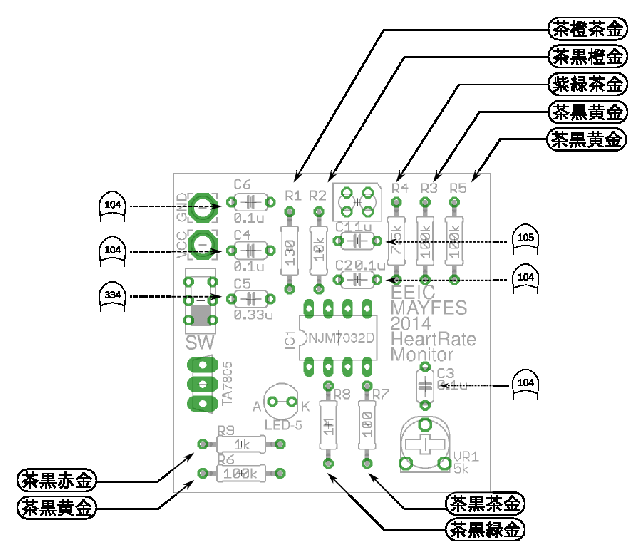
\includegraphics[width=9cm]{rc.eps}
 \caption{\small{抵抗、コンデンサの半田つけ}} 
\end{figure}
次にICやセンサといった部品、電源につなぐための導線を半田付けします。これらの部品には向きがあるので、必ず図2にか書かれている向きにあうように部品を差し込んでください。
\begin{figure}[H]
 \centering
 \small %8
 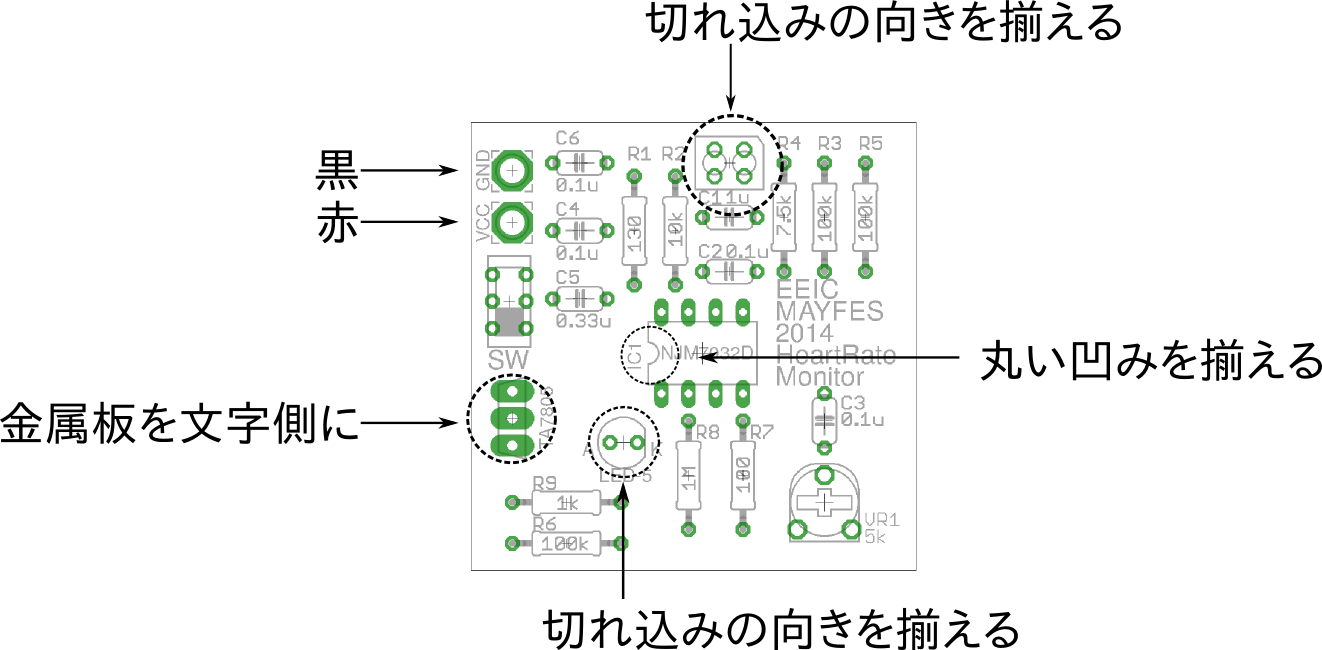
\includegraphics[width=12cm]{ic.eps}
 \caption{\small{ICの半田つけ}} 
\end{figure}

\newpage
\hspace{20mm}
\section{回路説明}
\hspace{20mm}
\begin{figure}[H]
 \centering
 \small %8
 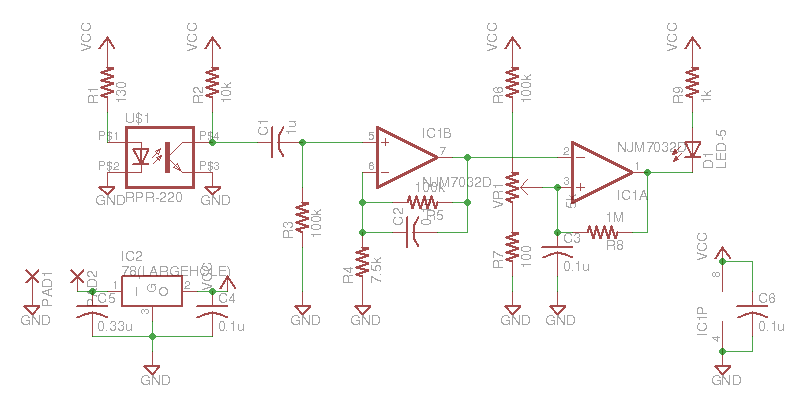
\includegraphics[width=12cm]{HeartRateMonitor_sch.eps}
 \caption{\small{回路図}} 
\end{figure}
図3が心拍数計の回路図です。この心拍数計は、血流が赤外線を吸収することを利用して、赤外線センサによって脈拍を検知しています。赤外線センサで検知した信号は、とても小さくて他の回路からは認識できないので、次の回路で脈拍の信号を増幅します。最後に増幅した信号をつかって信号があるかないかを判定して、LEDを点滅させています。信号の有る、無しを判断するしきい値は、回路に付けられているVR(半固定抵抗)という部品を回すことで設定します。

\end{document}

